%Styles
\tikzstyle{cog} = [draw=black, inner sep=0, minimum size = 0.2cm, circle, node distance=2cm, path picture={ 
      \filldraw[] (path picture bounding box.west) -- (path picture bounding box.east)-- (path picture bounding box.north east) -- (path picture bounding box.north) -- (path picture bounding box.south) -- (path picture bounding box.south west) -- cycle;}]
\tikzstyle{force}=[>=latex,draw=blue,fill=blue]
\tikzstyle{axis} =[dashed,gray,font=\small]

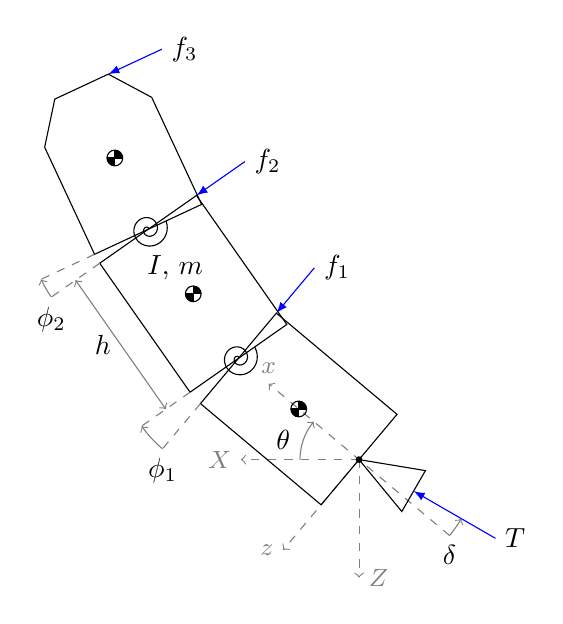
\begin{tikzpicture}[scale=1]
\def\h{2cm}
\def\w{1.5cm}
\def\thet{50}
\def\phio{-15}
\def\phit{-10}
\def\del{10}

%   Newtonian Ref frame 
 	\draw[axis,->]  (0,0) -- (0,-\w)  node[right]{$Z$};
 	\draw[axis,->]  (0,0) --  (-\w,0) node[left]{$X$};
 	\draw[draw=gray,->,] (-\w/2,0) node[above left]{$\theta$} arc (180 : 90+\thet : \w/2);
	
	\begin{scope}[yshift=0,rotate=\thet]
 	\draw[axis,->]  (0,-0.75*\h) -- (0,\w)  node[above]{$x$};
 	\draw[axis,->]  (0,0) --  (-\w,0) node[left]{$z$};
	\draw[] (-\w/2,0) rectangle (\w/2,\h);
	\node[cog] at (0,\h/2) {};	
	\draw[axis,-]  (-\w/2,\h) -- (-\w,\h);
	\draw[draw=gray,->,] (-\w,\h) node[below]{$\phi_1$} arc (180:180+\phio:\w);
	\draw[force,->] (\w,\h)  node[right]{$f_1$}  -- (\w/2,\h);
	
	\begin{scope}[yshift=\h,rotate=\phio]

	\draw[] (-\w/2,0) rectangle (\w/2,\h);
	\node[cog] at (0,\h/2) {};
	\node[] at  (0,0.7*\h) {$I$, $m$};
	\draw[axis,-]  (-\w/2,\h) -- (-\w,\h);
	\draw[axis,-]  (-\w/2,0) -- (-\w,0);
	\draw[draw=gray,->,] (-\w,\h) node[below]{$\phi_2$} arc (180:180+\phit:\w);
	\draw[force,->] (\w,\h)  node[right]{$f_2$}  -- (\w/2,\h);
	\draw [domain=0:12.56,variable=\t,smooth,samples=75] plot ({\t r}: {0.020*\t});
	\draw[draw=gray,<->,] (-0.75*\w,0)  -- node[left]{$h$} (-0.75*\w,\h);
	
	\begin{scope}[yshift=\h, rotate=\phit]
	\draw[axis,-]  (-\w/2,0) -- (-\w,0);
	\draw[] (-\w/2,0) -- (-\w/2,3*\h/4) -- (-\w/4,\h) -- (\w/4,\h) -- (\w/2,3*\h/4) -- (\w/2,0) --  (-\w/2,0) ;
	\node[cog] at (0,\h/2) {};	
	\draw[force,->] (3*\w/4,\h)  node[right]{$f_3$}  -- (\w/4,\h);
	\draw [domain=0:12.56,variable=\t,smooth,samples=75] plot ({\t r}: {0.020*\t});
	
	\end{scope}
	\end{scope}
	
	\begin{scope}[rotate = \del]
	\draw[]  (0,0) -- (-0.2*\w,-0.4*\h) -- (0.2*\w,-0.4*\h) -- cycle;
	\draw[force,->] (0,-\h)  node[right]{$T$}  -- (0,-0.4*\h);
	\filldraw (0,0) circle (1pt);
	\end{scope}
	\draw[draw=gray,->,] (0,-0.75*\h) node[below]{$\delta$} arc (-90:-90+\del:0.75*\h);

	\end{scope}


\end{tikzpicture}